\documentclass{article}
\usepackage[margin=2.54cm]{geometry}
\usepackage{graphicx}   % imágenes
\graphicspath{{img}}
\usepackage{amsfonts}   % fuentes de conjuntos numéricos
\usepackage{amsmath}
\usepackage{tikz}       % gráficos
\usepackage{pgfplots}   % plots
\pgfplotsset{width=10cm, compat=1.9}
\usepgfplotslibrary{external}
\tikzexternalize
\setlength{\jot}{8pt}
\setlength{\parindent}{0cm}
\usepackage{cancel}     % cancelar términos

\title{porfolio2}
\author{Daniel Ise}
\date{June 2024}

\begin{document}

\begin{titlepage}
    \begin{center}
        \vspace*{.5cm}
        \includegraphics[scale=.5]{img/udemm-logo.png}\\
        \vspace{.2cm}
        \Large
        \textbf{Facultad de Ingeniería}\\
        \textbf{Ingeniería en Sistemas}\\
        \vspace{2cm}

        \Huge
        Análisis de Sistemas II \\
        Examen Parcial I \\
        Iteración N\(^\circ\) 2 \\
        \vfill

        \raggedright
        \Large
        Docentes:
        \begin{itemize}
            \item[] Mg. Margarita Castronuovo \\
        \end{itemize}
        Alumno:
        \begin{itemize}
            \item[] Daniel Ise
        \end{itemize}
        Legajo:
        \begin{itemize}
            \item[] 28547
        \end{itemize}
        Fecha:
        \begin{itemize}
            \item[] Mayo, 2025
        \end{itemize}
    \end{center}
\end{titlepage}

\section*{Unidad 4: Derivadas y aplicaciones}
\subsection*{Actividad 1}

Modelo:

\begin{align*}
	h_{(t)} &= 40t - 5t^2
\end{align*}

\subsection*{1.A}

La velocidad media se puede obtener siguiendo la expresión:

\begin{align*}
	V_m &= \frac{h_{(t2)} - h_{(t1)}}{t_2 - t_1}
\end{align*}

Evaluando esta expresión para los intervalos solicitados obtenemos:

\begin{center}
\begin{tabular}{ c c }
	Intervalo	&	Velocidad Media \\
	\hline \\
	$[0, 2]$	&	30\\	
	$[1, 4]$	&	15\\
	$[4, 7]$	&	-15\\
	$[1, 7]$	&	0
\end{tabular}
\end{center}

\textbf{Conclusiones}

Como cabría esperar de un modelo de lanzamiento vertical, la velocidad media 
es inicialmente más alta, decrece con el paso el tiempo y 
pasa a ser negativa en el tercer intervalo considerado. 
El cuarto intervalo la piedra se ubica a la misma altura en los segundos 1 y 7,
dando con ello una velocidad media de 0, aunque la piedra se encuentra en 
movimiento en ambos instantes.

\subsection*{Actividad 1.B}

\begin{center}
\begin{tikzpicture}
	\draw[->] (0, 0) -- (8, 0) node[right] {$x$};
	\draw[->] (0, 0) -- (0, 8) node[above] {$y$};
	\draw[scale=0.1, domain=0:8, smooth, variable=\x, blue] plot ({\x},{\x*40-\x*\x*5});
	\filldraw[black] (0,0) circle (2pt) node[anchor=east]{$(0, 0)$};
	\filldraw[black] (0.8,0) circle (2pt) node[anchor=north]{$(8, 0)$};
	\filldraw[black] (0.4,8) circle (2pt) node[anchor=west]{$(4, 80)$};
\end{tikzpicture}
\end{center}


\subsection*{1.C}

La información que brinda la velocidad media en el intervalo $[1, 7]$ es insuficiente para calcular la velocidad en $t=2$, así como en $t=4$, puesto que es igual a 0. Para conocer la velocidad en esos instantes es preciso determinar la derivada de la función que, como dijimos en el apartado anterior, es $h'_{(t)}=40-10t$. Con esta expresión es posible calcular la velocidad instantánea en todo el dominio de la función considerada.
\input{01/02actividad}
\subsection*{3}

Modelos de automóvil 1 y 2.

\begin{align*}
    D_1 &= t &
    D_2 &= \frac{t^2}{2}
\end{align*}

\input{01/03partea}
\subsubsection*{Parte B}

\begin{center}
\begin{tikzpicture}
\begin{axis}[
    axis lines = left,
    xlabel = \(t\),
    ylabel = {\(D(t)\)},
    clip = false,
]

% D_2
\addplot[
    domain=0:3,
    samples=200,
    color=cyan,
]
{x*x/2};
\addlegendentry{\(D_2=\frac{t^2}{2}\)}

% Derivada que pasa por 2
\addplot[
    domain=1:3,
    samples=200,
    color=orange,
]
{2*x-2};
\addlegendentry{\(D'_2=2t-2\)}

\node[label={270:{(2,2)}},circle,fill,inner sep=2pt] at (axis cs:2,2) {};

\end{axis}
\end{tikzpicture}
\end{center}

Para obtener la función que describe a la recta tangente a la función en el punto $(2, 2)$ expresamos este punto en la notación punto-pendiente, incluyendo como pendiente al valor devuelto por la derivada de $D_2$, que en ese punto es 2. Entonces:

\begin{align*}
    y-2 &= 2(x-2)\\
    y &= 2x - 4 + 2\\
    y &= 2x - 2
\end{align*}

Por otra parte, para obtener la función que describe la recta secante correspondiente al intervalo $[1,5; 2]$, calculamos en primer lugar su pendiente:

\begin{align*}
    m &= \frac{D_{2(2)} - D_{2(1,5)}}{2 - 1,5}\\
    m &= \frac{2 - 9/8}{2 - 1,5}\\
    m &= \frac{7}{4}
\end{align*}

Con la expresión de la pendiente, tomamos uno de los puntos por el cual deseamos que cruce, en este caso puede ser $(2, 2)$, y planteamos la función en notación punto-pendiente:

\begin{align*}
    y-2 &= \frac{7}{4}(x-2)\\
    y &= \frac{7}{4}x - \frac{7}{2} + 2\\
    y &= \frac{7}{4}x - \frac{3}{2}
\end{align*}

Con la expresión $y = \frac{7}{4}x - \frac{3}{2}$, podemos representar la secante.

\begin{center}
\begin{tikzpicture}
\begin{axis}[
    axis lines = left,
    xlabel = \(t\),
    ylabel = {\(D(t)\)},
    clip = false,
]

% D_2
\addplot[
    domain=1:3,
    samples=200,
    color=cyan,
]
{x*x/2};
\addlegendentry{\(D_2=\frac{t^2}{2}\)}

% Secante que pasa por 2
\addplot[
    domain=1.5:2,
    samples=200,
    color=magenta,
]
{7/4*x-3/2};
\addlegendentry{\(S=\frac{7}{4}t - \frac{3}{2}\)}

\node[label={270:{(2,2)}},circle,fill,inner sep=2pt] at (axis cs:2,2) {};
\node[label={270:{(1,5,9/8)}},circle,fill,inner sep=2pt] at (axis cs:1.5,1.125) {};
\end{axis}
\end{tikzpicture}
\end{center}

\begin{center}
\begin{tabular}{ c c c c c c c c c c c c }
    t & 1,5 & 1,9 & 1,99 & 1,999 & 1,9999 & 2 & 2,0001 & 2,001 & 2,01 & 2,1 & 2,5\\
	\hline \\
    $g_{(t)} = \frac{t^2}{2}$ & 1.125 & 1.805 & 1.98 & 1.998 & 1.9998 & 2 & 2.0002 & 2.002 & 2.02 & 2.205 & 3.125 \\
    \vspace{10pt} \\
    $\frac{g_(t) - g_(2)}{t - 2}$ & 1.75 & 1.95 & 2 & 2 & 2 & 2 & 2 & 2 & 2 & 2.05 & 2.25\\
    \vspace{10pt} \\
    \hline
\end{tabular}
\end{center}

Como puede observarse tanto en las gráficas como en la tabla construida, a medida que los extremos de la recta secante se aproximan, el valor de su pendiente tiende al valor de la derivada en dicho punto.
\section*{Actividad 2}

Para aproximarnos al problema de la princesa Dido desde la optimización, podemos imaginar una elipse, cuyos semiejes denominaremos $a$ y $b$.

\begin{center}
    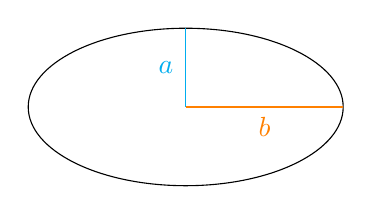
\begin{tikzpicture}
        \draw (0,0) ellipse (2cm and 1cm);
        \draw[-, cyan] (0,0) -- (0,1); % línea a
        \draw[cyan] (-0.25,0.5) node{$a$}; % label a
        \draw[-, orange] (0,0) -- (2,0); % línea b
        \draw[orange] (1,-0.25) node{$b$}; % label b
    \end{tikzpicture}
\end{center}

Podemos plantear dos ecuaciones, una para su área:

\begin{align*}
    A &= \pi ab
\end{align*}

Y otra para su perímetro:

\begin{align*}
    P &= \pi (a + b)
\end{align*}

En nuestro caso, el perímetro funciona como una restricción, a partir de la cual podemos despejar $a$, para expresar el área del elipse en función de $b$:

\begin{align*}
    \pi (a + b) &= 100\\
    a &= \frac{100}{\pi} - b
\end{align*}

Expresamos el área en función de $b$:

\begin{align*}
    A &= \pi b (\frac{100}{\pi} - b)\\
    A &= 100b - \pi b^2
\end{align*}

Derivamos esta función:

\begin{align*}
    \frac{dA}{dx} &= 100 - 2 \pi b
\end{align*}

E igualamos a 0, para determinar el punto máximo de la función del área:

\begin{align*}
    100 - 2 \pi b &= 0\\
    b &= \frac{-100}{-2 \pi}\\
    b &= \frac{50}{\pi}
\end{align*}

De ahí determinamos que $a$ es: 

\begin{align*}
    a &= \frac{100}{\pi} - \frac{50}{\pi}\\
    a &= \frac{50}{\pi}\\
    a &= b
\end{align*}

La elipse cuyos semiejes son iguales, en este caso $a$ y $b$, es el círculo. El círculo sería entonces la figura que maximizaría el área.

\section*{Unidad 5: Integrales y aplicaciones}

\subsection*{Métodos de integración}

\begin{figure}
    \centering
    \includegraphics[width=20cm, angle=270]{img/metodos integracion.png}
    \caption{Métodos de Integración}
    \label{fig:metodos-integracion}
\end{figure}

\begin{figure}
    \centering
    \includegraphics[width=22cm, angle=270]{img/integracion por fracciones parciales.png}
    \caption{Integración por fracciones parciales}
    \label{fig:integracion-fracciones-parciales}
\end{figure}

\include{02/02ParteB}
\end{document}
